\documentclass[a4paper, 12pt]{article}

% NOTE: packates que se usaran en todo el proyecto
% paquetes para el idioma
\usepackage[T1]{fontenc}
\usepackage[spanish]{babel}
\defineshorthand{"-}{\babelhyphen{hard}} % para que los guiones o dashes no se fusionen

\usepackage[utf8]{inputenc}

\usepackage[top=25mm, left=25mm, bottom=25mm, right=18mm, headheight=25mm, b5paper]{geometry}

\usepackage{graphicx} % Imagenes
\usepackage{parskip} % Arreglo de la tabulación en el documento
\usepackage{xcolor, soul} % Para poder usar colores
\usepackage{titletoc} % Para personalizar la tabla de contenido
\usepackage{titlesec} % Para personalizar los títulos de los capítulos y las secciones
\usepackage{textcomp} % Agrega el paquete textcomp en el preámbulo
\usepackage{fancyhdr} % Para trabajar con el encabezado
\usepackage{amssymb} % Agrega el paquete amssymb en el preámbulo
\usepackage{listings} % Para usar el paquete listings y sintaxis de códigos
\usepackage{lipsum} % para generar texto aleatorio
\usepackage{booktabs} % Para usar tablas personalizadas.
\usepackage{lmodern} % Latin moderno
 % packages

\graphicspath{{./assets/}}



\begin{document}

\begin{center}
	\huge\textbf{\textblue{Clean Code JavasCript}}

	% 
\includegraphics[width=10cm]{banner} % Logo de Lua
	\vspace{0.5cm} % space
\end{center}

\section{Introducción}

\begin{center}
  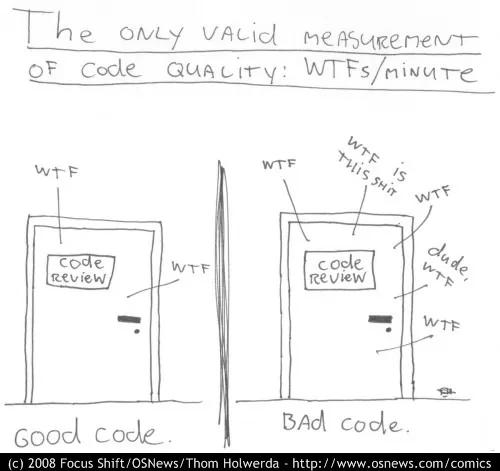
\includegraphics[width=12cm]{introduction_bad_code} % Logo de Lua
	\vspace{0.5cm} % space
\end{center}

Los principios de la ingeniería de software, del libro de Robert C. Martin \textblue{\textit{Clean Code}}, adaptado para JavasCript. Esta no es una guía de estilo, en cambio, es una guía para crear software que sea reutilizable, comprensible y que se pueda mejorar con el tiempo.

No hay que seguir tan estrictamente todos los principios en este libro, y vale la pena mencionar que hacia muchos de ellos habrá controversia en cuanto al consentimiento. Estas son reflexiones hechas después de muchos años de experiencia colectiva de los autores de \textit{Clean Code}.

Una cosa más: saber esto no te hará un mejor ingeniero inmediatamente, y tampoco trabajar con estas herramientas durante muchos años garantiza que nunca te equivocarás. Cualquier código empieza primero como un borrador, como arcilla mojada moldeándose en su forma final. Por último, arreglamos las imperfecciones cuando lo repasamos con nuestros compañeros de trabajo. No seas tan duro contigo mismo por los borradores iniciales que aún necesitan mejorar. ¡Trabaja más duro para mejorar el programa!

\newpage

\section{Variables}

\subsection*{Utiliza nombres significativos y pronunciables para las variables}

Mal Hecho:
\begin{lstlisting}[language=TypeScript, style=badstyle]
 const yyyymmdstr = moment().format('YYYY/MM/DD');
\end{lstlisting}
\vspace{0.5cm} % space

Bien Hecho:
\begin{lstlisting}[language=TypeScript, style=goodstyle]
 const fechaActual = moment().format('YYYY/MM/DD');
\end{lstlisting}

\subsection*{Utiliza el vocabulario igual para las variables del mismo tipo}

Mal Hecho:
\begin{lstlisting}[language=TypeScript, style=badstyle]
 conseguirInfoUsuario();
 conseguirDataDelCliente();
 conseguirRecordDelCliente();
\end{lstlisting}
\vspace{0.5cm} % space

Bien Hecho:
\begin{lstlisting}[language=TypeScript, style=goodstyle]
 conseguirUsuario();
\end{lstlisting}

\subsection*{Utiliza nombres buscables}

Nosotros leemos mucho más código que jamás escribiremos. Es importante que el código que escribimos sea legible y buscable. Cuando faltamos nombrar a las variables de manera buscable y legible, acabamos confundiendo a nuestros lectores. Echa un vistazo a las herramientas para ayudarte: \textblue{\underline{buddy.js}} y \textblue{\underline{ESLint}}.

Mal Hecho:
\begin{lstlisting}[language=TypeScript, style=badstyle]
 // Para que rayos sirve 86400000?
 setTimeout(hastaLaInfinidadYMasAlla, 86400000);
\end{lstlisting}
\vspace{0.5cm} % space

Bien Hecho:
\begin{lstlisting}[language=TypeScript, style=goodstyle]
 // Declaralos como variables globales de 'const'.
 const MILISEGUNDOS_EN_UN_DIA = 8640000;

 setTimeout(hastaLaInfinidadYMasAlla, MILISEGUNDOS_EN_UN_DIA);
\end{lstlisting}

\newpage

\subsection*{Utiliza variables explicativas}

Mal Hecho:
\begin{lstlisting}[language=TypeScript, style=badstyle]
 const direccion = 'One Infinite Loop, Cupertino 95014';
 const codigoPostalRegex = /^[^,\\]+[,\\\s]+(.+?)\s*(\d{5})?$/;
 saveCityZipCode(direccion.match(codigoPostalRegex)[1], direccion.match(codigoPostalRegex)[2]);
\end{lstlisting}
\vspace{0.5cm} % space

Bien Hecho:
\begin{lstlisting}[language=TypeScript, style=goodstyle]
 const direccion = 'One Infinite Loop, Cupertino 95014';
 const codigoPostalRegex = /^[^,\\]+[,\\\s]+(.+?)\s*(\d{5})?$/;
 const [, ciudad, codigoPostal] = direccion.match(codigoPostalRegex) || [];
 guardarcodigoPostal(ciudad, codigoPostal);
\end{lstlisting}

\subsection*{Evitar el mapeo mental}

El explícito es mejor que el implícito.

Mal Hecho:
\begin{lstlisting}[language=TypeScript, style=badstyle]
 const ubicaciones = ['Austin', 'New York', 'San Francisco'];
 ubicaciones.forEach((u) => {
   hazUnaCosa();
   hasMasCosas()
   // ...
   // ...
   // ...
   // Espera, para que existe la 'u'?
   ejecuta(u);
 });
\end{lstlisting}
\vspace{0.5cm} % space

Bien Hecho:
\begin{lstlisting}[language=TypeScript, style=goodstyle]
 const ubicaciones = ['Austin', 'New York', 'San Francisco'];
 ubicaciones.forEach((ubicacion) => {
   hazUnaCosa();
   hazMasCosas()
   // ...
   // ...
   // ...
   ejecuta(ubicacion);
 });
\end{lstlisting}

\newpage

\subsection*{No incluyas contexto innecesario}

Si el nombre de tu clase/objeto te dice algo, no lo repitas de nuevo en el nombre de variable.

Mal Hecho:
\begin{lstlisting}[language=TypeScript, style=badstyle]
 const Coche = {
   cocheMarca: 'Honda',
   cocheModelo: 'Accord',
   cocheColor: 'Blue'
 };

 function pintarCoche(coche) {
   coche.cocheColor = 'Red';
 }
\end{lstlisting}
\vspace{0.5cm} % space

Bien Hecho:
\begin{lstlisting}[language=TypeScript, style=goodstyle]
 const Coche = {
   marca: 'Honda',
   modelo: 'Accord',
   color: 'Blue'
 };

 function pintarCoche(coche) {
   coche.color = 'Red';
 }
\end{lstlisting}

\subsection*{Utiliza argumentos predefinidos en vez de utilizar condicionales}

Los argumentos predefinidos muchas veces son más organizados que utilizar los condicionales. Se consciente que si tú los usas, tu función sólo tendrá valores para los argumentos de \lineCode{undefined}. Los demás valores de 'falso' como \lineCode{\textquotesingle\textquotesingle}, \lineCode{\textquotedblright\textquotedblright}, \lineCode{false}, \lineCode{null}, \lineCode{0} y \lineCode{NaN}, no se reemplazan con un valor predefinido.

Mal Hecho:
\begin{lstlisting}[language=TypeScript, style=badstyle]
 function crearEmpresa(nombre) {
   const nombreEmpresa = nombre || 'Tacos S.A';
   // ...
 }
\end{lstlisting}
\vspace{0.5cm} % space

Bien Hecho:
\begin{lstlisting}[language=TypeScript, style=goodstyle]
 function crearEmpresa(nombreEmpresa = 'Tacos S.A') {
   // ...
 }
\end{lstlisting}

\newpage

\section{Funciones}

\subsection*{Argumentos de funciones (2 o menos idealmente)}

Limitar la cantidad de parámetros de tus funciones es increíblemente importante ya que hace que tus pruebas del código sean más fáciles. Al pasar los 3 argumentos, llegarás a un escenario de una explosión combinatoria en que hay que comprobar con pruebas muchos casos únicos con un argumento separado.

Uno o dos argumentos es la situación ideal, y más que eso uno debe evitar si es posible. Todo lo que se puede consolidar se debe consolidar. Normalmente, si tienes más que dos argumentos, tu función sirve para hacer demasiado. En otros casos, es mejor refactorizar y hacerlo un objeto para encapsular las funciones extras.

Ya que JavaScript te deja crear objetos cuando quieras sin incorporar la arquitectura de 'clases', se puede usar un objeto si necesitas muchos argumentos.

Para hacerlo más obvio cuáles argumentos espera la función, se puede usar la sintaxis de ES2015/ES6: 'destructuración'. Esta sintaxis tiene varias ventajas:









Mal Hecho:
\begin{lstlisting}[language=TypeScript, style=badstyle]
\end{lstlisting}
\vspace{0.5cm} % space

Bien Hecho:
\begin{lstlisting}[language=TypeScript, style=goodstyle]
\end{lstlisting}

\end{document}
